\chapter[AM generation using IFT]{AM generation using IFT}

\section*{Aim}
To design and set-up  an AM generator using BJT and IFT and measure the modulation index from the observed output waveform.

\section*{Theory}
Any amplifier can be converted into a sinusoidal oscillator if Barkhausen conditions are satisfied. So tuned amplifier in chapter \ref{iftamplifier} can be converted ito a high frequency oscillator for generating carrier wave by providing a positive feedback after removing  the input and the load resistor $R_L$.

Inorder to obtain the feedback signal to the base, the terminal-1 of the IFT primary coil is used. It is $180^{\circ}$ out of phase with the signal at collector, ie. terminal-2 of IFT primary winding. The collector signal is already $180^{\circ}$ out of phase with the signal at base of BJT. Thus the feed back signal from terminal-1 of the IFT to the base of BJT is in phase with the signal at the base. The feedback capacitor is chosen to be low to avoid additional phase shift.  

The circuit now works as an oscillator generating a signal of frequency of around 455 kHz. Its amplitude, $E_c$ can be slightly adjusted by varying the potentiometer connected in series with the emitter resistance and frequency, $f_c$ by tuning the IFT.
\begin{equation}
e_c\ =\ E_c\ sin(2\pi f_ct)
\end{equation}
The carrier thus generated can be modulated using an audio frequency message signal by connecting it at the emitter of the transistor. It can be of frequency varying from 1kHz to 5 kHz. The amplitude can be varied in the rage of 1 V to 10 V which changes the modulating index.


\paragraph{}
The ratio of the maximum amplitude of the modulating signal voltage to that of the carrier voltage is termed as modulation index. This is represented as $m=\frac{E_m}{E_c}$. For both carrier and message being sinusoidal, the modulation index will be 
$m=\frac{E_{max}-E_{min}}{E_{max}+E_{min}}$
\noindent where $E_{max}$ and $E_{min}$ are respectively the maximum and minimum height of the positive side of modulated signal.
\section*{Design}
The basic biasing of the transistor is as discussed in the chapter \ref{iftamplifier}.\\
To make the circuit an oscillator, remove input and the load.\\
Positive feed back signal to base is taken from terminal-1 of IFT and given to base through a small capacitance of $C_1=100 pF$. \\
The emitter resistance can be raplaced with a fixed resistance of $R_E=1k\Omega$ in series with a potentiometer of $R_3=5k\Omega$.\\
The modulating signal is connected through a capacitor of $C_E=10\mu F$.
\section*{Circuit Diagram}
The circuit diagram is shown in Fig. \ref{amiftpng}
\begin{figure}
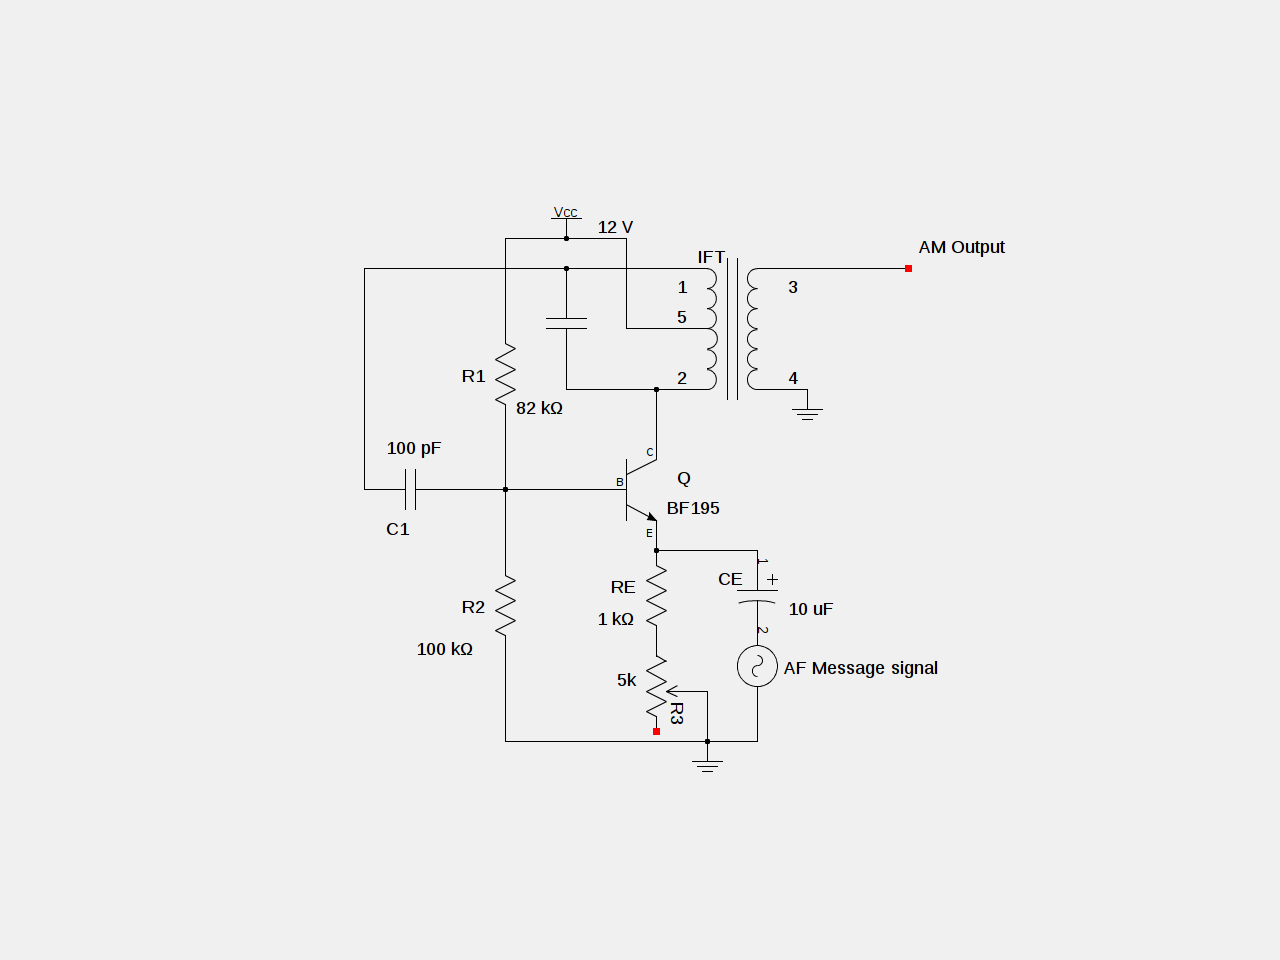
\includegraphics[width=\textwidth, height=9cm, trim=9cm 5cm 8cm 6cm,clip=true]{amift.png}
\caption{Circuit Diagram for AM generation using IFT}
\label{amiftpng}
\end{figure}
\section*{Procedure}

\begin{enumerate}
\item
Set up the circuit after verifying the condition of components.
\item
Feed AF modulating signal (say, $f_m=1kHz$ and $E_m=5mV$) using a function generator.
\item
Adjust amplitude and frequencies of the AF and carrier signals and observe amplitude modulated waveform on the CRO.
\item
Fix $f_m$ and $f_c$. Note down $E_{max}$ and $E_{min}$ of the AM signal and calculate modulation index according to the formula ,
\begin{equation}
m=\frac{E_{max}-E_{min}}{E_{max}+E_{min}}.
\end{equation}
Here $E_{max}$ is the maximum of the positive envelope of the carrier and $E_{min}$ is the minimum of the positive envelope of the carrier.
\item
Repeat for different values of $E_m$ and $E_c$. Observe the AM waveforms for different values of m.
\item
Plot the waveforms on a graph sheet.
\item

Fill in the observation column
\end{enumerate}


\section*{Observation}


\begin{figure}[h]

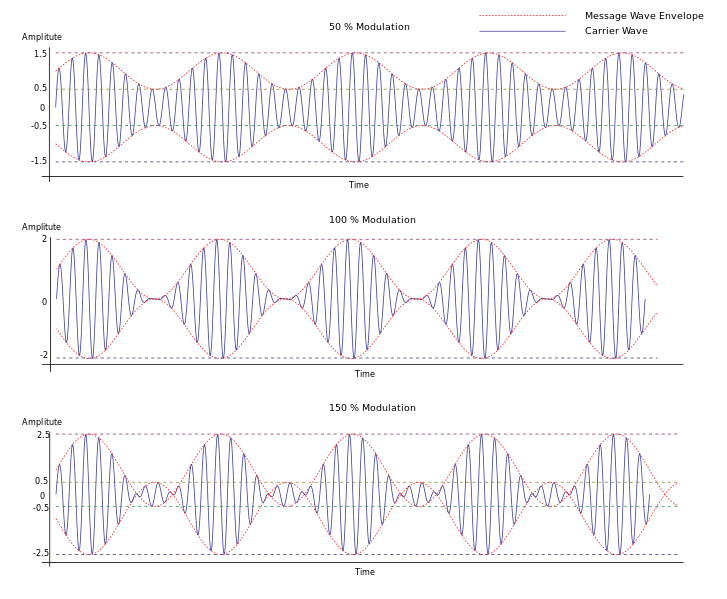
\includegraphics[width=\textwidth,height=12cm]{AMmodindex.png}
\caption{Effect of modulation index on AM}
\label{AMmodindex1}
\end{figure}
\noindent Figure. \ref{AMmodindex1}  shows the effect of modulation index on the resultant AM wave\footnote{Image source: \url{https://commons.wikimedia.org:/wiki/File:Amplitude_Modulated_Wave-hm-64.svg}}
\begin{center}

\begin{tabular}{|l|l|l|}

\hline
 & &\\
 
$E_{min}$  & $E_{max}$ & $m=\frac{E_{max}-E_{min}}{E_{max}+E_{min}}$ \\
 & & \\ \hline
 & & \\ \hline
& & \\ \hline
& & \\ \hline


\end{tabular}
\end{center}
\section*{Result}
Implemented the AM modulation circuit using BJT and IFT. Tabulated the modulation index by varying the amlitudes of message and the carrier.

